\chapter{SciCheck: Completing scientific Knowledge Graphs}\label{chap:scicheck}

\chapterQuote{
    \hfill
    \foreignlanguage{russian}{\sffamily доверяй, но проверяй.}\\
    \null
    \hfill
    \textit{(Trust, but verify.)}
}{--- Russian proverb}

\chapterAbstract{S}{cientific knowledge is in constant expansion, and many efforts have been developed throughout the years to capture it in a structured format. Knowledge Graphs can support this task, by linking entities representing research concepts together. These scientific KGs have particular nuances that make completing them a particularly challenging task. In this chapter, we introduce SciCheck, our proposal to complete Knowledge Graphs representing research concepts. This chapter is structured in the following manner: Section~\ref{sec:sci-intro} provides an introduction, Section~\ref{sec:sci-proposal} describes SciCheck in detail, including the features that it uses to characterize triples representing scientific knowledge, Section~\ref{sec:sci-evaluation} presents the experimental evaluation that we have carried out to assess its efficacy and efficiency in practice, Section~\ref{sec:sci-aikg} shows a practical application of SciCheck on AI-KG, a large-scale Knowledge Graph of research concepts and, finally, Section~\ref{sec:sci-summary} provides a summary of the chapter.}

\section{Introduction}\label{sec:sci-intro}
% In recent years, we have witnessed the appearance of a number of Knowledge Graphs that represent research and scientific knowledge. These graphs are generally either manually curated~\cite{jaradeh2019, bodenreider2004, kuhn2016}, or constructed automatically from academic metadata~\cite{dessi2020aikg, salatino2020, rossanez2020}. However, just like most KGs, they suffer from incompleteness, which means that some well-known scientific knowledge may not be present in them.

% This chapter introduces SciCheck~\cite{borrego2022}, our proposal to complete scientific Knowledge Graphs. SciCheck extends our generic triple classification technique, CAFE, by adding a number of features and heuristics specifically tailored for the scientific domain. SciCheck is able to compute a confidence score for every triple representing a scientific claim, and then derive a binary classification for it based on its confidence. Similarly to CAFE, SciCheck works by transforming a triple into numeric features, but includes additional heuristics to immediately discard incorrect scientific triples.

% We evaluate the efficacy of SciCheck on seven different Knowledge Graphs and against nine alternative approaches to this task. Our evaluation shows that SciCheck is able to obtain a significantly better precision than its state-of-the-art counterparts, which is of the essence to reliably extend scientific Knowledge Graphs.

% Additionally, we used SciCheck to extend the Artificial Intelligence Knowledge Graph (AI-KG)~\cite{dessi2020aikg}, a large-scale open KG that is constructed automatically using the 300K most cited papers in the field of Artificial Intelligence. Initially, AI-KG contained 1.2M statements about scientific claims in this field. By applying SciCheck to it, we have expanded it with 300K additional high-confidence statements. This application has resulted in the release of a new, expanded version of AI-KG, as well as in the creation of two high-quality Knowledge Graphs that can be used to benchmark KG completion.

\section{Our proposal}\label{sec:sci-proposal}
% SciCheck is a triple classification technique specifically designed to complete scientific statements in a Knowledge Graph. It is an extension of the CAFE approach~\cite{borrego2021} that incorporates a new set of features and heuristics that are specifically tailored to capture scientific knowledge. 

% SciCheck takes an entire KG in the form of triples as input, and produces one neural-based classifier for each relation in the KG as output. Specifically, given a relationship $r$, SciCheck generates a model $f_r : (s,r,t) \rightarrow c$, that assigns a confidence score $c$ in the range $[0,1]$ to any arbitrary triple $(s,r,t)$ to solve a binary classification task (``is the triple correct or not?''). To feed the models, triples are converted into a numerical vector representation using ad-hoc features and contextual embedding representations. SciCheck can operate on any KG and focuses on optimizing precision, to ensure that the knowledge deemed correct is trustworthy.

% In the following, we describe and discuss the features that SciCheck uses to characterize a triple in the context of a scientific KG.

% \begin{figure}[!htp]
%     \centering
%     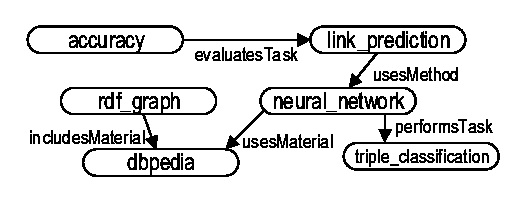
\includegraphics[width=.55\textwidth]{fig/scicheck/example_kg}
%     \caption{A small KG with research information about the Semantic Web}
%     \label{fig:example-kg-sw}
% \end{figure}

% For the sake of illustration, Figure \ref{fig:example-kg-sw} displays a small KG that will be used to provide specific examples.

\subsection{Extended feature set}
% SciCheck uses an extensible set of features specifically made to capture and process scientific information, which represent the neighborhoods of the two entities of a triple in a variety of ways. Each triple is evaluated by all features. Additionally, each feature can also depend on a number of parameters, such as a maximum neighborhood size. 

% Since, as described, SciCheck is an extension of CAFE, we enumerate only the additional features that it incorporates with respect to the original CAFE approach.

% \scifeature
% {Cosine similarity of the word embeddings of the source and target entities}
% {This feature measures the semantic similarity of the two entities in a triple, using any entity embeddings. If we consider $A$ and $B$ to be the embeddings of the source and target entities of the triple respectively, it is defined as:}
        
% \[
%     \cos (A, B) = 
%     \frac{ \sum_{i=1}^{n}{{A}_i{B}_i} }{ \sqrt{\sum_{i=1}^{n}{({A}_i)^2}} \sqrt{\sum_{i=1}^{n}{({B}_i)^2}} }
% \]

% \scifeature
% {Dot product of the word embeddings of the source and target entities}
% {This feature complements the previous one by also taking into account the magnitudes of the embeddings of the entities. If we consider $A$ and $B$ to be the embeddings of the source and target entities of the triple respectively, it is defined as:}

% \[
%     A \cdot B = \sum_{i=1}^{n}{A_i B_i}
% \]

% \newpage

% \scifeature
% {Types of the source and target entities according to the ontology of the Knowledge Graph}
% {This feature encodes the known types of the entities according to the available ontology as two one-hot vectors. In Figure \ref{fig:example-kg-sw}, the entity \textit{dbpedia} is of type \textit{Resource}, while \textit{accuracy} is a \textit{Metric}.}


% Regarding the rationales of the new features, $f_1$ incorporates information from the word embeddings of the two entities, which have been shown to be advantageous for triple classification \cite{sun2019, kazemi2018}. SciCheck uses by default the \roberta{} model \cite{liu2019roberta} to generate the word embeddings, since is able to capture and represent semantic similarities across a wide range of domains. Similarly, $f_2$ provides a similar assessment, but uses the magnitudes of the embedding vectors to extract additional information from them.

% Feature $f_3$ leverages the ontological schema of the KG. This allows SciCheck to include information regarding the types of the two entities in a triple into the feature vector for that triple. Furthermore, SciCheck can automatically classify a triple as incorrect if the triple does not respect the domains and ranges of the relation as defined in the ontological schema. For example, in the KG shown in Figure~\ref{fig:example-kg-sw}, the triple \textit{(accuracy, evaluatesTask, rdf\_graph)} would be considered incorrect without further evaluation, because the range of the relation \textit{evaluatesTask} is the type \textit{Task}, while \textit{rdf\_graph} is a \textit{Material}. 

% This extension of the set of features allows SciCheck to better characterize scientific entities and predicates. In particular, the features based on word embeddings enable SciCheck to exploit the implicit contextual information from the training papers that may not be encoded in the KG.
% Additionally, the inclusion of ontology-based features allows SciCheck to take advantage of the available high-level knowledge about any specific domain. These improvements are particularly crucial for assessing scientific claims, which tend to use a specific jargon and to rely on a well-defined epistemological framework.

% Furthermore, different types of relations in the graph may carry specific insight that should be captured separately. For this reason, SciCheck first computes all features in the input KG as-is, and then it computes them again in different versions of the KG where only relations of a single type are present. This is done for all the different relations in the KG. Additionally, in features that use the neighborhoods of the source and target entities, such as those originally defined by CAFE, these two neighborhoods are calculated using all possible combinations of relations. Finally, SciCheck concatenates all the resulting features in the final feature vector. The features which involve computing entity neighborhoods or paths use a maximum neighborhood size for their computations. Following the findings in \cite{borrego2021}, by default SciCheck computes them for a maximum size of 1, 2, and 3. The resulting set of features using different neighborhood sizes are eventually all added to the final feature vector. 


\section{Evaluation}\label{sec:sci-evaluation}
% In this section, we describe the experimental setup that we devised to test the effectiveness of SciCheck in practice. First, we introduce a number of similar state-of-the-art approaches to triple classification that serve as baselines for our evaluation. Next, we present the KGs that we used to validate our proposal. Finally, we show and discuss the results of our evaluation.

\subsection{Baselines}
% We evaluated the performance of SciCheck against a number of alternative approaches. Five of the baselines are well-known embedding-based KG completion techniques: \textit{TransE}~\cite{bordes2013}, \textit{TransD}~\cite{ji2015}, \textit{TransH}~\cite{wang2014}, \textit{SimplE}~\cite{kazemi2018}, and \textit{ComplEx}~\cite{trouillon2016}. To provide a common ground to train and test these techniques, we used the OpenKE \cite{han2018} tool.

% In order to better assess the contributions of the different components of SciCheck, we also considered five alternative versions of our approach:

% \begin{itemize}
%     \item \textit{CAFE Baseline}, which uses solely the context-aware features for KG completion such as neighborhood size, shared entities and connectivity from the original CAFE implementation \cite{borrego2021}.\\
    
%     \item \textit{CAFE+\roberta}, which extends CAFE by considering features based on the similarity of the embeddings of the source and target entities, using the RoBERTa model.\\
    
%     \item \textit{CAFE+SciBERT}, which extends CAFE by considering features based on the similarity of the embeddings of the source and target entities, using SciBERT, an alternative BERT-based text embedding model~\cite{reimers2019} specifically tailored to scientific documents.\\
    
%     \item \textit{CAFE+Ontology}, which extends CAFE by considering features that identify the types of the source and target entities according to the domain ontology and also filters triples whose entities are not consistent with the domain and range restrictions of the relation.\\
    
%     \item \textit{SciCheck}, the full version of our approach, which incorporates both features based on word embeddings and features based on the ontology of the Knowledge Graph.
% \end{itemize}

% To predict the correctness of a triple using SciCheck, we convert its confidence score in the interval $[0, 1]$ into a binary label by setting a confidence threshold for a correct triple of 0.5, as suggested in~\cite{borrego2021}. The thresholds of the other state-of-the-art techniques under evaluation and their results were obtained using the OpenKE tool, allowing it to choose the optimal value for each one.

\subsection{Evaluation data}
% The previously discussed baselines were evaluated on the following Knowledge Graphs, whose characteristics are summarized in Table~\ref{table:sci-dsets}:

% \begin{table}[!htp]
    % \footnotesize
    \begin{center}
    \begin{tabular}{ >{\raggedright\arraybackslash}M{2.5cm} | M{1.75cm} | M{1.75cm} | M{1.5cm} | M{1.5cm} }
    \hline\rule{0pt}{12pt}
    \textbf{KG} & \textbf{Training triples} & \textbf{Test triples} & \textbf{Entities} & \textbf{Relations} \\
    
    \hline%
    AIKG-1M & 860,512 & 430,280 & 820,708 & 20 \\ 
    AIKG-500 & 860,512 & 500 & 228 & 7 \\ 
    FB13 & 228,172 & 105,509 & 74,998 & 13 \\ 
    WN11 & 77,948 & 36,042 & 38,195 & 9 \\
    WN18 & 71,984 & 33,282 & 40,943 & 11 \\
    WN18RR & 86,835 & 3,134 & 40,943 & 11 \\
    NELL & 86,971 & 40,104 & 53,934 & 148  \\ \hline
    \end{tabular}
    \caption{Overview of the KGs used for evaluating SciCheck}
    \label{table:sci-dsets}
    \end{center}
\end{table}
    

% \begin{itemize}
%     \item \textit{AIKG-1M}, a new KG that we created from AI-KG. We used a de-reified version of AI-KG, in order to consider only triples which involve tasks, methods, materials, metrics, and other scientific entities. As a result, 1,075,652 triples were directly generated from scientific literature, without considering facts that were materialized using the domain semantics defined in the AI-KG ontology (e.g., transitivity). Triples were split into a training and a testing set with a split ratio of 80\%-20\%, respectively.
%     To generate negative triples in the testing split, each positive triple was corrupted once by randomly replacing the target entity with another one within the domain of the relation in the triple, i.e., if the range of the target entity is a Task, then it is substituted by another entity whose type is Task. We also make sure that the randomly generated negative triple is not already present in the KG, to prevent creating false negatives whenever possible. As an example, the triple \textit{(dbpedia, usesOtherEntity, sparql\_query)} is correct, while the corrupted version \textit{(dbpedia, usesOtherEntity, cost\_function)} is considered incorrect, where \textit{sparql\_query} and \textit{cost\_function} are both of type \textit{OtherEntity}. However, negative examples were not generated for the training split, as specific KG completion techniques usually have a preferred way to generate them automatically \cite{borrego2019}. In total, the training split comprised 860,512 positive triples and the testing split includes 430,280 triples ($50\%$ positive and $50\%$ negative).\\

%     \item \textit{AIKG-500}, a new KG that we constructed by manually annotating triples in AI-KG about the Semantic Web. 
%     To construct it, we randomly selected 250 triples which had as their source entity one of the 24 sub-topics of the Semantic Web according to the CSO ontology \cite{salatino2020CSO} and were considered to be correct by at least 2 methods among \textit{TransE}, \textit{TransD}, \textit{TransH}, \textit{SimplE}, \textit{ComplEx}, and \textit{SciCheck}. Another 250 triples were randomly selected out of those deemed incorrect by at least 2 of the previously mentioned techniques. The resulting 500 triples were manually annotated by five domain experts, with an inter-reviewer agreement of 0.61 (according to Cohen's kappa), which is typically considered a substantial agreement.
%     A majority vote approach was used to determine that 221 triples were correct and 279 were incorrect. Since this Knowledge Graph was created for the purpose of providing a small but high-quality and  manually-annotated testing split, in this evaluation we used AIKG-1M for the training split.\\

%     \item \textit{FB13} \cite{socher2013}, a subset of FreeBase~\cite{bollacker2008} that focuses on relevant people and their family relations, locations, professions, and other personal data.\\
        
%     \item \textit{WN11} \cite{bordes2013}, a subset of WordNet centered around different semantic relations between over 38K words.\\
        
%     \item \textit{WN18} \cite{bordes2014}, which expands WN11 with additional relations.\\
    
%     \item \textit{WN18RR} \cite{dettmers2018}, which improves WN18 by removing reciprocal relations in the test set. This makes triple classification more challenging, since otherwise the model can predict that a triple \textit{(a, hasChildren, b)} is true whenever the triple \textit{(b, hasParent, a)} appears in the training set.\\
        
%     \item \textit{NELL} \cite{gardner2015}, a subset of the NELL KG~\cite{mitchell2018} with information and relations about many different domains, e.g., actors which starred in movies, writers and their works, or athletes and their teams.\\
% \end{itemize}

% It is well-known \cite{dettmers2018} that these traditional KGs suffer from information leakage between the training and test sets, due to the presence of reciprocal relations. For this reason, we removed all reciprocal relations in all KGs except WN18, since we also include its previously discussed sanitized version, WN18RR.

% \subsection{Results and discussion}\label{sec:sci-results}
% Table~\ref{fig:sci-table_p} and Table~\ref{fig:sci-table_r} report the precision and recall of the KG completion techniques on AIKG-1M. The results show that all CAFE-based variants outperform embedding-based techniques in precision, achieving notably higher values. Including features from the text embeddings also provides an important improvement over the base version of CAFE. Both SciCheck and the variants that improve the baseline using embedding-based features rank consistently among those with the highest precision for all relations, with the differences between them being very narrow.

% \begin{figure}[!h]
%     \centering
%     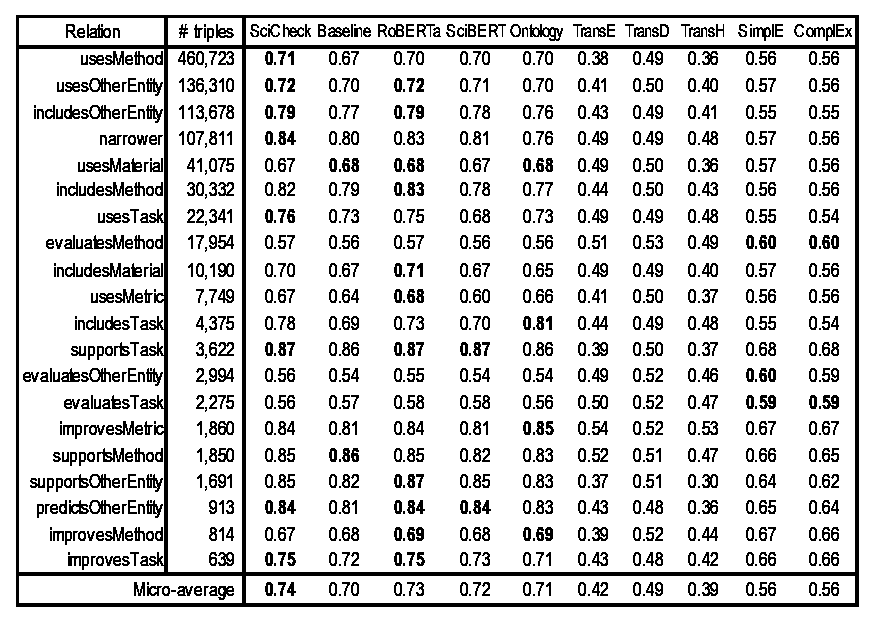
\includegraphics[width=\textwidth]{fig/scicheck/table_p}
%     \captionof{table}{Precision values for SciCheck in AIKG-1M}
%     \label{fig:sci-table_p}
% \end{figure}

% \begin{figure}[!h]
%     \centering
%     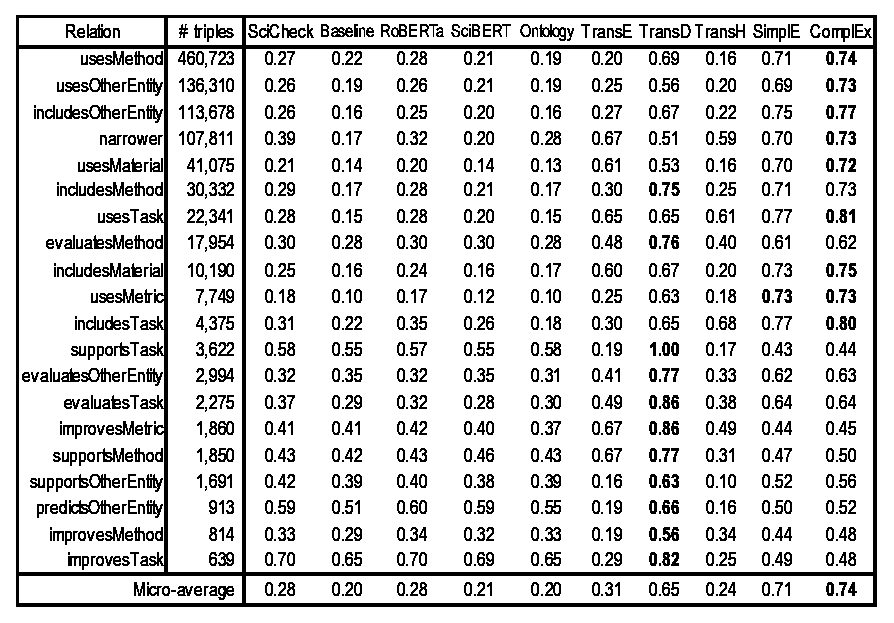
\includegraphics[width=\textwidth]{fig/scicheck/table_r}
%     \captionof{table}{Recall values for SciCheck in AIKG-1M}
%     \label{fig:sci-table_r}
% \end{figure}

% The best performing method in terms of precision is the full version of SciCheck (0.74), followed by CAFE+\roberta{} (0.73), which can obtain better precision for some less common relationships. 
% Interestingly, using text embeddings trained specifically on academic abstracts (SciBERT) yields a slightly worse performance than using the generic \roberta{} model. This may suggest that more general embeddings may sometimes produce better performance on KGs of research concepts, but this needs to be investigated further.

% The \textit{Ontology} variation, which includes one-hot type vectors and domain/range checking for the relation, only slightly improves the baseline. This is most likely due to the type-constrained way in which the negative triples were generated, since it already guarantees that the domain and range types of the relation are preserved.

% The recall of SciCheck is naturally lower than that of the embedding-based approaches, in a typical precision-recall trade-off. However, this is acceptable since the main goal is to expand scientific Knowledge Graphs with correct triples, hence, a high precision is desirable. SciCheck also has a generally higher recall than all other CAFE variants. Consequently, the results suggest that SciCheck is the best performing technique for the task of reliably completing scientific Knowledge Graphs.

% It is noteworthy that different relations can lead to very different performances. For instance, relations such as \textit{narrower}, \textit{supportsTask} and \textit{supportsMethod} yield very good performance. Conversely, the methods under evaluation did not perform as well on relations such as  \textit{evaluatesTask} and \textit{evaluatesOtherEntity}. This may depend on the number of relevant examples or the fact that some relations are inherently harder to predict.

% In order to study the performance of the different techniques for all possible threshold values, we also report their corresponding ROC curves in Figure~\ref{fig:sci-rocs}. This analysis confirms the previous findings:  

% \begin{itemize}
%     \item SciCheck outperforms all other methods under evaluation.
%     \item Text embedding-based features significantly improve the baseline state-of-the-art methods.
%     \item Ontology-based features provide slight further improvements.
% \end{itemize}

% In addition, Figure~\ref{fig:sci-rocs-embs} confirms that SciCheck outperforms the standard state-of-the art methods regardless of the threshold.

% \begin{figure}[!htp]
%     \centering
%     \def\subfw{0.45\textwidth}
    
%     \subfigure[SciCheck variants]{
%         \includesvg[inkscapelatex=false, width=\subfw]{fig/scicheck/roc_cafes.svg}
%         \label{fig:sci-roc-cafes}
%     }~
%     \subfigure[SciCheck and embedding techniques]{
%         \includesvg[inkscapelatex=false, width=\subfw]{fig/scicheck/roc_embs.svg}
%         \label{fig:sci-rocs-embs}
%     }
    
%     \caption{ROC curves of the different methods on AIKG-1M}
%     \label{fig:sci-rocs}
% \end{figure}

% To check whether the differences between the methods were statistically significant, we used DeLong's test~\cite{delong1988} to compare the areas under two curves. The p-values obtained when comparing the ROC  curve of SciCheck with the alternative methods in Figures~\ref{fig:sci-roc-cafes} and~\ref{fig:sci-rocs-embs} were all~$<0.0001$. This very high statistical confidence is due to the large number of observations, since the testing set of AIKG-1M includes more than 400,000 triples.

% Table~\ref{fig:sci-table_sw} shows the performance of the methods on AIKG-500, which are consistent with the previous findings. For the sake of brevity, here we do not report the results of all CAFE variants, which are in line with those obtained on AIKG-1M. Even in a smaller, manually annotated Knowledge Graph, SciCheck achieves a high precision, which confirms that it is suitable for completing scientific Knowledge Graphs. 

% \begin{figure}[!htp]
%     \centering
%     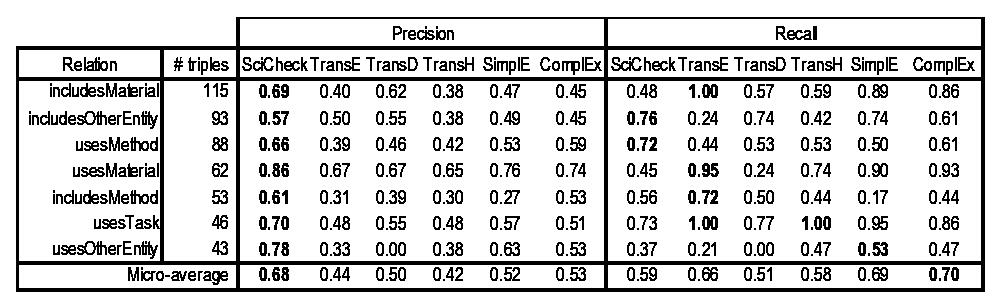
\includegraphics[width=\textwidth]{fig/scicheck/table_sw}
%     \captionof{table}{Precision and recall values for AIKG-500}
%     \label{fig:sci-table_sw}
% \end{figure}

% Table~\ref{fig:sci-table_kgs} reports the performance of all the techniques on five standard KGs for triple classification. The results show that SciCheck is able to outperform other techniques in almost all cases, thus being an effective triple classification tool for KGs of many different natures. They also confirm that completing scientific KGs is indeed a challenging task that requires specialized techniques, as the general-purpose embedding-based approaches yield worse results on KGs extracted from AI-KG in comparison to generic ones.

% \begin{table}[!htp]
%     \centering
%     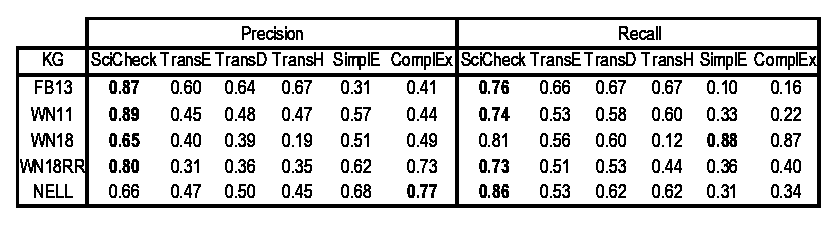
\includegraphics[width=.85\textwidth]{fig/scicheck/table_kgs}
%     \captionof{table}{Micro-average precision and recall on four general KGs}
%     \label{fig:sci-table_kgs}
% \end{table}

% In order to assess the scalability of our solution, Table~\ref{table:sci-times} reports the seconds used by SciCheck to process the previously discussed graphs. To ensure statistical significance, we measured the runtime for each KG 10 times, and we report the average and the standard deviation for each one. 

% \begin{table}[!htp]
    % \footnotesize
    \begin{center}
    \begin{tabular}{ M{2.5cm} | M{3.5cm} }
    \hline\rule{0pt}{12pt}
    \textbf{KG} & \textbf{Runtime}  \\
    
    \hline%
    AIKG-1M & 2,758.79 $\pm$ 37.27 \\ 
    AIKG-500 & 1,794.94 $\pm$ 12.58 \\ 
    FB13 & 9,400.10 $\pm$ 63.04 \\ 
    WN11 & 34.30 $\pm$ 0.28 \\
    WN18 & 55.59 $\pm$ 0.45  \\
    WN18RR & 26.00 $\pm$ 0.14 \\
    NELL & 4.33 $\pm$ 0.09 \\ \hline
    \end{tabular}
    \caption{SciCheck runtimes in seconds for all KGs (avg $\pm$ std)}
    \label{table:sci-times}
    \end{center}
\end{table}

% Table \ref{table:sci-times} shows that the runtime ranges from a few seconds to over two hours according to the specific Knowledge Graph. These differences are caused by mainly two factors. First, the amount of distinct entities corresponds directly to the number of \roberta{} embeddings that have to be computed, which are typically quite time-consuming. Hence, a larger number of entities has a negative impact on runtime. Second, and most importantly, the specific topology of every KG affects the size of the neighborhoods of the entities, and thus also affects the time it takes to compute features on them. The case of FB13 is particularly noteworthy since, in contrast with the other KGs, it contains many entities with a very high cardinality. This causes the sizes of the entity neighborhoods to grow exponentially in size, resulting in longer runtimes.

% Finally, in order to provide some insights on how these times compare to other state-of-the-art approaches, Table~\ref{table:sci-times-comp} reports their runtime in seconds compared to that of SciCheck for AIKG-1M.

% \begin{table}[!htp]
    % \footnotesize
    \begin{center}
    \begin{tabular}{ M{2.5cm} | M{3.5cm} }
    \hline\rule{0pt}{12pt}
    \textbf{Technique} & \textbf{Runtime}  \\
    
    \hline%
    SciCheck & 2,758.79 \\ 
    TransE & 7,147.52 \\ 
    TransD & 13,871.79 \\ 
    TransH & 10,134.41 \\
    SimplE & 6,592.20 \\
    ComplEx & 11,767.73 \\ \hline
    \end{tabular}
    \caption{Runtime comparison on AIKG-1M}
    \label{table:sci-times-comp}
    \end{center}
\end{table}
    

% Embedding-based KG completion approaches were run using $1,000$ iterations, as it is commonly done in related literature~\cite{bordes2013, trouillon2016, kazemi2018, ji2015}. 
% SciCheck took considerably less time to run on the large AIKG-1M KG than its state-of-the-art counterparts. This suggests that it is able to complete scientific facts in a reasonable amount of time, thus making it efficient for its application to large-scale scientific Knowledge Graphs.

\section{Practical application: AI-KG}\label{sec:sci-aikg}
% One practical application of SciCheck is the advancement and expansion of AI-KG~\cite{dessi2020aikg}, a comprehensive Knowledge Graph that encompasses information about research entities in the AI field. When it was introduced in late 2020, it contained roughly 14 million RDF triples and 1.2 million reified statements related to 800,000 entities extracted from 333,000 articles about AI. It defines 5 categories of entities (tasks, methods, materials, metrics, and others) connected by 27 relations (e.g., usesMaterial, evaluatesMethod, or supportsTask). The triples in AI-KG illustrate the associations between two entities based on their joint appearances in a group of scientific papers, for instance, \textit{(sentiment\_analysis, usesMaterial, twitter\_data)}.

% It should be emphasized that, in the context of AI-KG, the correctness of a triple depends on the content of its associated papers, i.e., a triple connected to a group of papers is considered to be true if said papers contain that statement. As a result, triples in AI-KG are constructed to represent particular statements made by researchers. For instance, the entity \textit{sentiment\_analysis} only captures the notion of sentiment analysis that existed in the original corpus of scientific articles on which AI-KG was built, and does not attempt to encompass all existing techniques for analyzing emotions and sentiments that are present, or under research, nowadays. A complete representation of such information would require elevating research entities into more abstract elements representing ontological knowledge, which is currently beyond the intended scope of AI-KG.

% AI-KG was constructed by extracting entities and their relations from a corpus of scientific articles using Natural Language Processing (NLP) and Machine Learning (ML) techniques \cite{dessi2021generating}, using the following data pipeline:

% \begin{enumerate}
%     \item Entity detection and extraction using transformer-based, domain-specific extractors \cite{wadden2019}.
%     \item Entity classification into the CSO ontology \cite{salatino2019}.
%     \item Relation detection and extraction through a number of NLP and ML techniques \cite{wadden2019, angeli2015,toutanova2003}.
%     \item Fact identification and validation using AI-KG's own ontology.%\footnote{\url{http://scholkg.kmi.open.ac.uk/aikg/ontology}}.
%     \item Fact ranking using the number of research papers that contain the fact as a measurement of support.
% \end{enumerate}

% The interested reader can find the fine-grained steps of this process in the relevant literature \cite{dessi2020aikg,dessi2021generating}. At the time of the application of our technique, the entities contained within AI-KG were classified into one of the following types:

% \begin{itemize}
%     \item \textit{Task}: A specific challenge or piece of work to be completed as part of a research project.
%     \item \textit{Method}: A proposed approach or plan for accomplishing a research task.
%     \item \textit{Material}: Resources that are utilized for a research task, such as a dataset, image, or text corpus.
%     \item \textit{Metric}: Entities that can be measured and are used to evaluate the effectiveness of a research method.
%     \item \textit{OtherEntity}: A category that encompasses entities that do not fit into any of the previous terms.
% \end{itemize}

% The relations were created by clustering frequent verbs together, and asking human experts to define domain, range, and transitiveness restrictions. Some examples of object properties are \textit{evaluatesMethod}, \textit{includesMaterial}, or \textit{usesMethod}.

% AI-KG is currently in use by a number of organizations due to its ability to store structured information about the AI field, and has supported other related research, for example, entity extraction in the context of scientific articles \cite{li2021}, classifying such articles \cite{hoppe2021}, and describing and managing competencies \cite{heist2021}.

% Despite AI-KG being a large-scale Knowledge Graph, extracting unstructured knowledge from natural language is a difficult and error-prone task. For this reason, AI-KG does not cover all well-known facts in the AI domain, either because they were not detected or not extracted correctly. As a consequence, AI-KG, as most automatically generated Knowledge Graphs, is incomplete. An example of this is the absence of the triple \textit{(neural\_network, usesMaterial, rdf\_graph)} from AI-KG, even though RDF graphs are used as input for most of the neural network-based techniques that perform link prediction or triple classification, for example, CAFE.

% Because of this, scientific Knowledge Graphs require specific methods for their completion \cite{jaradeh2021}. Nevertheless, the most well-known methods that work on general-purpose Knowledge Graphs, like TransE, TransR, or RotatE, have not been successful in predicting triples with a high precision in AI-KG. As discussed in Section~\ref{sec:sci-results}, even though these methods provide reasonable F1 values, they yield low precision values (usually between 40-60\%). Applying these existing methods would lead to a considerable amount of inaccurate information being introduced in AI-KG. This, in turn, has been the motivation for this particular use case.

% We applied SciCheck to AI-KG and, by setting a confidence threshold of $0.7$, generated $303,760$ new high-confidence facts. To do this, we used SciCheck to connect the most popular 500 entities that meet the domain and range restrictions imposed by the AI-KG ontology for every relation. As a result, many significant triples representing well-known facts that were missed by AI-KG's NLP extraction pipeline were materialized, such as:

% \begin{center}
%     \textit{(search\_engine, includesMaterial, knowledge\_base)}\\
%     \textit{(f\_measure, evaluatesMethod, neural\_network)}\\
%     \textit{(neural\_network, usesMaterial, rdf\_graph)}\\
%     \textit{(recommender\_system, usesMethod, predictive\_model)}
% \end{center}

% We collaborated with the original authors of AI-KG to make this improved version available online at \url{https://zenodo.org/record/7276434}. 

% \section{Summary}\label{sec:sci-summary}
% In this chapter we introduced SciCheck, our proposal for scientific Knowledge Graph completion. SciCheck extends CAFE by adding a number of features specifically tailored for the scientific domain, namely, measuring the similarity of the embedded representations of two concepts in a certain way, as well as representing and applying ontological constraints on what is considered correct knowledge.

% We have performed an extensive evaluation, comparing SciCheck with other state-of-the-art approaches and analyzing its individual components. The results show that SciCheck is able to classify triples representing scientific knowledge with a considerably higher precision than its counterparts, and that it is also more efficient in practice, requiring shorter runtimes than other proposals.

% Finally, we have applied SciCheck to the large-scale AI-KG Knowledge Graph, which contains more than 1.2 million facts about the Artificial Intelligence domain. As a result of this process, we have expanded AI-KG with more than 300,000 additional high-confidence statements. In cooperation with the original authors of AI-KG, we have publicly released this improved version of it to the scientific community.